\chapter{User Documentation}

\section{System Requirements}

All of the code is written for \Csh 6.0. The \path{HexMage.GUI} project runs on Windows under .NET framework 4.5 (or newer). It also requires up to date graphics drivers, and optionally audio drivers when running with \texttt{--EnableAudio=true}. The experiments in \path{HexMage.Benchmarks} can be run on Linux under a recent version of Mono (tested on 4.x). See \autoref{sec:compilation} for more detailed instructions on how to compile and run the project.

\section{Generating Experiment Data}

The data for our survey are under the \path{data/manual-teams} directory. Each file represents a single team for which a suitable opponent will be generated by our algorithm. Any number of files can be added.

In order to generate the data for the experiment, simply run the \path{HexMage.Benchmarks.exe} program with no command line arguments (preferably in Release mode) and everything will be generated automatically. The results are stored under \path{data/questionnaire} in separate files in the DNA file format \autoref{dna-format}. Generating the data takes around 1 hour on Intel i7-5820k Processor \citep{intel-ark}. We've disabled parallelization in order to make the data generation deterministic and the whole experiment reproducible. An initial seed is defined under \verb|Constants.RandomSeed| and is used by all of the internal random number generators. Parallel execution can be re-enabled by defining a compile time \verb|PARALLEL| constant.

\section{Running the Experiment}

Running the \path{HexMage.GUI.exe} program will run the experiment by default. It loads the data from \path{data/questionnaire} and presents a list of the required games on the main screen (see \autoref{fig:questionnaire}). The state of the questionnaire is maintained in the files themselves. Specifically, finished games will be renamed to have a \path{.done} extension. This allows the user to resume at any point in time, and also makes it easy to revert back to an initial state if something goes wrong. Pressing \verb|Ctrl-Q| will reset all of the games to unplayed state. This is meant mostly for debugging.

The next game can be started by pressing \verb|Spacebar|, which immediately picks the next game on the list and loads it. After the game is finished, the questionnaire is opened in the default browser and the game identifier is pre-filled (we used Google Forms). The form itself is configured in \verb|QuestionnaireScene.cs|. After the user finishes playing the game, they should quit the program and re-launch it to proceed to the next game. We did this for stability purposes since the questionnaire was run remotely and we had no way to assist the user in case of errors.

We also provide the exact ZIP file we used to run the experiment with all of the generated games to make it easy to reproduce the results without having to run the encounter generation script.

\begin{figure}[h]
	\centering
	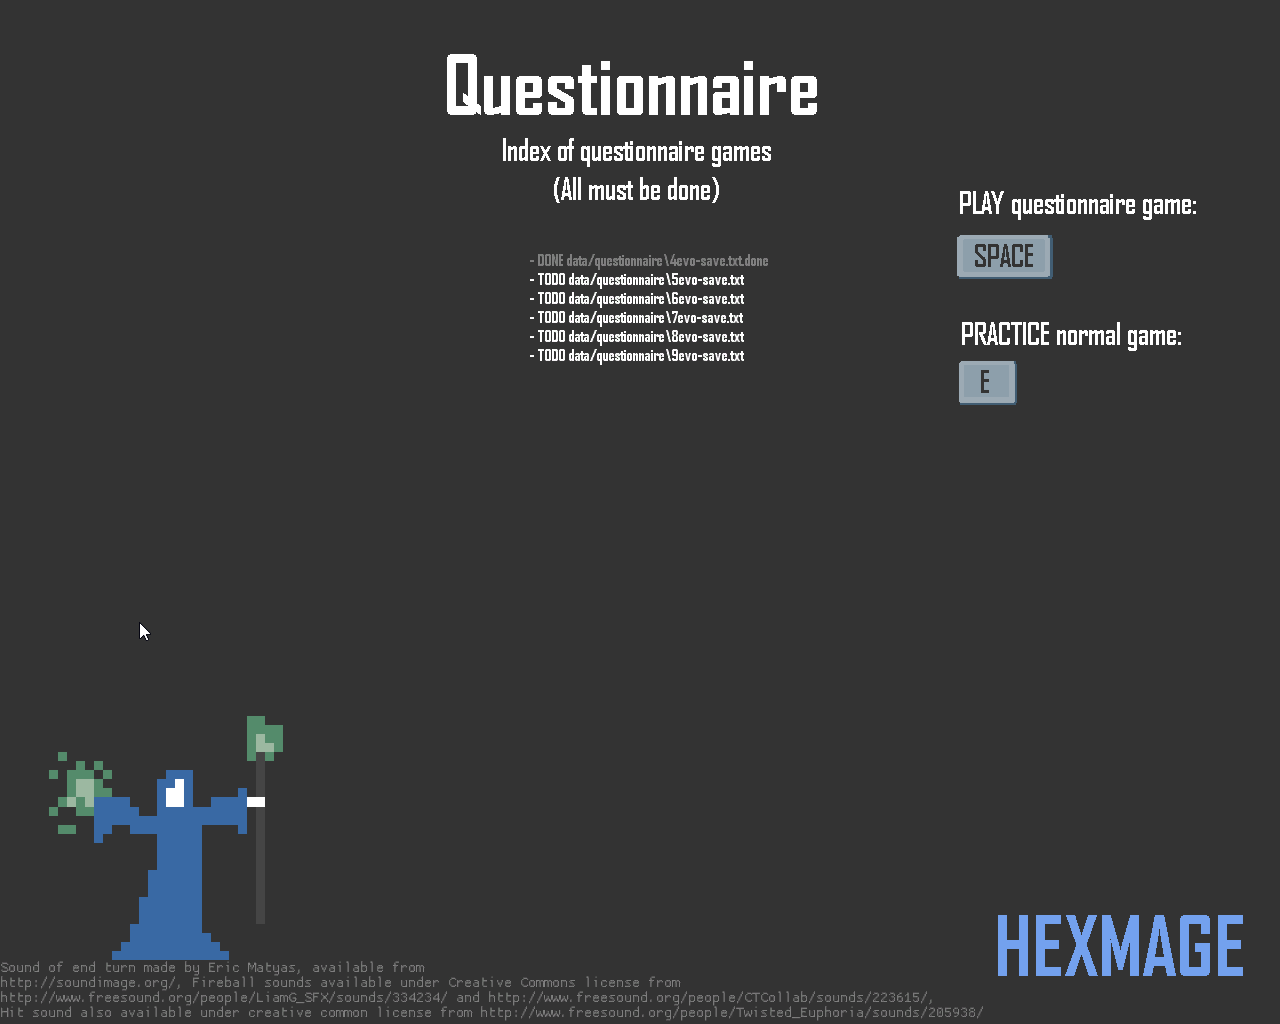
\includegraphics[width=0.95\textwidth]{img/questionnaire.png}
	\label{fig:questionnaire}
	\caption{The main screen of the questionnaire. It shows a list of games which must be played, along with their status. Finished games are displayed in gray and have a \emph{.done} extension, unfinished games are displayed in white. A keyboard shortcut information is also showed.}
\end{figure}

\section{Playing Custom Games}

The user can also press \verb|E| on the initial screen to go into \emph{Practice mode}. This opens up a map editor (see \autoref{fig:map-editor}) where the user can create a custom map, save it to a JSON file (see \autoref{map-format}), load saved files, set startup positions, and continue to the AI selection by pressing \verb|Space|. This allows the user to select AIs for both of the teams and set the team sizes (see \autoref{fig:team-selection}). At any point the user can press \verb|Ctrl-R| to go back to the initial scene. This can be done in game as well.

\begin{figure}
	\centering
	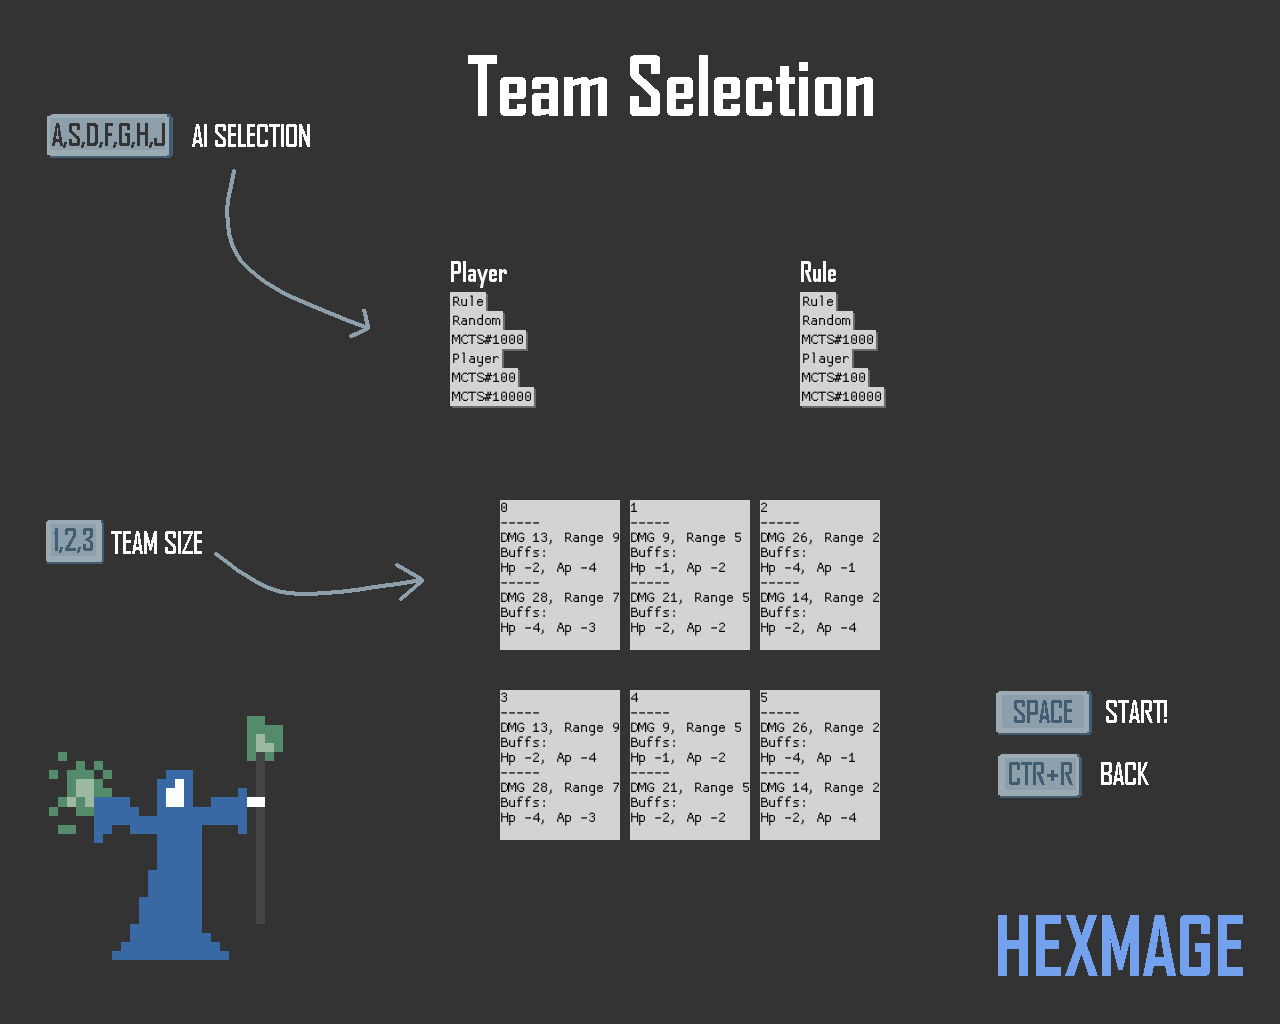
\includegraphics[width=0.95\textwidth]{img/team-selection.png}
	\label{fig:team-selection}
	\caption{Team selection scene which allows the user to pick AIs and team sizes before starting the game. The controls are described on the game screen.}
\end{figure}

Once the user is happy with the team selection, they can press \verb|Space| to start the game, which brings them to the arena scene (see \autoref{fig:arena}). It shows the current game state in the middle of the screen, abilities of the current mage on the left, abilities of the mage under the mouse cursor on the right, the current team at the top, the game history in bottom left, and the detail of a hex under the mouse cursor on the bottom right. Since there is no hidden information, the player can easily see what abilities his opponents have. \autoref{fig:cooldown-no-ap} shows the images representing different ability states. The currently active mage has their underlying hex colored in yellow.

When no ability is selected, the player moves his current mage by clicking the left mouse button on an empty hex. The game displays the distance to the hex in the bottom right corner, as well as drawing the path the mage will walk on. If the target hex is a wall or an enemy is standing on it, the path is not shown, indicating that the mage can not move to the target hex.

Abilities can be selected either by clicking on them with the left mouse button, or with the number keys on the keyboard (\verb|1| for the first, \verb|2| for the second, etc.). When an ability is active, it is shown glowing as shown in \autoref{fig:cooldown-no-ap}. With an active ability, the player can left-click on an enemy mage to use the ability on him. A visiblity indicator is drawn when hovering over an enemy to show whether the enemy is in range and the ability can be used on him.

After the player is finished with his turn, they can press \verb|Space| to finish the turn and move on to the next character.

\begin{figure}
	\centering
	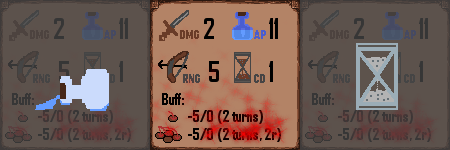
\includegraphics[width=0.60\textwidth]{img/cooldown-no-ap.png}
	\label{fig:cooldown-no-ap}
	\caption{(\emph{Left}) An image shown when the mage does not have enough action points for the given ability. (\emph{Middle}) An image of the currently selected and active ability. (\emph{Right}) An image shown when the given ability is on cooldown.}
\end{figure}